%%%%%%%%%%%%%%%%%%%%%%%%%%%%%%%%%%%%%%%%%%%%%%%%%%%%%%%%%%%%%%%%%%%%%%%%%%%%%%%%
%Tutorial slides on Python.
%
% Author: FOSSEE
% Copyright (c) 2009, FOSSEE, IIT Bombay
%%%%%%%%%%%%%%%%%%%%%%%%%%%%%%%%%%%%%%%%%%%%%%%%%%%%%%%%%%%%%%%%%%%%%%%%%%%%%%%%

\documentclass[14pt,compress]{beamer}
%\documentclass[draft]{beamer}
%\documentclass[compress,handout]{beamer}
%\usepackage{pgfpages} 
%\pgfpagesuselayout{2 on 1}[a4paper,border shrink=5mm]

% Modified from: generic-ornate-15min-45min.de.tex
\mode<presentation>
{
  \usetheme{Warsaw}
  \useoutertheme{infolines}
  \setbeamercovered{transparent}
}

\usepackage[english]{babel}
\usepackage[latin1]{inputenc}
%\usepackage{times}
\usepackage[T1]{fontenc}

% Taken from Fernando's slides.
\usepackage{ae,aecompl}
\usepackage{mathpazo,courier,euler}
\usepackage[scaled=.95]{helvet}
\usepackage{amsmath}

\definecolor{darkgreen}{rgb}{0,0.5,0}

\usepackage{listings}
\lstset{language=Python,
    basicstyle=\ttfamily\bfseries,
    commentstyle=\color{red}\itshape,
  stringstyle=\color{darkgreen},
  showstringspaces=false,
  keywordstyle=\color{blue}\bfseries}

%%%%%%%%%%%%%%%%%%%%%%%%%%%%%%%%%%%%%%%%%%%%%%%%%%%%%%%%%%%%%%%%%%%%%%
% Macros
\setbeamercolor{emphbar}{bg=blue!20, fg=black}
\newcommand{\emphbar}[1]
{\begin{beamercolorbox}[rounded=true]{emphbar} 
      {#1}
 \end{beamercolorbox}
}
\newcounter{time}
\setcounter{time}{0}
\newcommand{\inctime}[1]{\addtocounter{time}{#1}{\tiny \thetime\ m}}

\newcommand{\typ}[1]{\lstinline{#1}}

\newcommand{\kwrd}[1]{ \texttt{\textbf{\color{blue}{#1}}}  }

%%% This is from Fernando's setup.
% \usepackage{color}
% \definecolor{orange}{cmyk}{0,0.4,0.8,0.2}
% % Use and configure listings package for nicely formatted code
% \usepackage{listings}
% \lstset{
%    language=Python,
%    basicstyle=\small\ttfamily,
%    commentstyle=\ttfamily\color{blue},
%    stringstyle=\ttfamily\color{orange},
%    showstringspaces=false,
%    breaklines=true,
%    postbreak = \space\dots
% }

%%%%%%%%%%%%%%%%%%%%%%%%%%%%%%%%%%%%%%%%%%%%%%%%%%%%%%%%%%%%%%%%%%%%%%
% Title page
\title[Solving Equations \& ODEs]{Python for Science and Engg:\\Solving Equations \& ODEs}

\author[FOSSEE] {FOSSEE}

\institute[IIT Bombay] {Department of Aerospace Engineering\\IIT Bombay}
\date[] {14 December, 2009\\Day 1, Session 6}
%%%%%%%%%%%%%%%%%%%%%%%%%%%%%%%%%%%%%%%%%%%%%%%%%%%%%%%%%%%%%%%%%%%%%%

%\pgfdeclareimage[height=0.75cm]{iitmlogo}{iitmlogo}
%\logo{\pgfuseimage{iitmlogo}}


%% Delete this, if you do not want the table of contents to pop up at
%% the beginning of each subsection:
\AtBeginSubsection[]
{
  \begin{frame}<beamer>
    \frametitle{Outline}
    \tableofcontents[currentsection,currentsubsection]
  \end{frame}
}

\AtBeginSection[]
{
  \begin{frame}<beamer>
    \frametitle{Outline}
    \tableofcontents[currentsection,currentsubsection]
  \end{frame}
}

% If you wish to uncover everything in a step-wise fashion, uncomment
% the following command: 
%\beamerdefaultoverlayspecification{<+->}

%\includeonlyframes{current,current1,current2,current3,current4,current5,current6}

%%%%%%%%%%%%%%%%%%%%%%%%%%%%%%%%%%%%%%%%%%%%%%%%%%%%%%%%%%%%%%%%%%%%%%
% DOCUMENT STARTS
\begin{document}

\begin{frame}
  \maketitle
\end{frame}

%% \begin{frame}
%%   \frametitle{Outline}
%%   \tableofcontents
%%   % You might wish to add the option [pausesections]
%% \end{frame}

\section{Solving linear equations}

\begin{frame}[fragile]
\frametitle{Solution of equations}
Consider,
  \begin{align*}
    3x + 2y - z  & = 1 \\
    2x - 2y + 4z  & = -2 \\
    -x + \frac{1}{2}y -z & = 0
  \end{align*}
Solution:
  \begin{align*}
    x & = 1 \\
    y & = -2 \\
    z & = -2
  \end{align*}
\end{frame}

\begin{frame}[fragile]
\frametitle{Solving using Matrices}
Let us now look at how to solve this using \kwrd{matrices}
  \begin{lstlisting}
    In []: A = array([[3,2,-1],
                      [2,-2,4],                   
                      [-1, 0.5, -1]])
    In []: b = array([[1], [-2], [0]])
    In []: x = solve(A, b)
  \end{lstlisting}
\end{frame}

\begin{frame}[fragile]
\frametitle{Solution:}
\begin{lstlisting}
In []: x
Out[]: 
array([[ 1.],
       [-2.],
       [-2.]])
\end{lstlisting}
\end{frame}

\begin{frame}[fragile]
\frametitle{Let's check!}
\begin{lstlisting}
In []: Ax = dot(A,x)
In []: Ax
Out[]: 
array([[  1.00000000e+00],
       [ -2.00000000e+00],
       [  2.22044605e-16]])
\end{lstlisting}
\begin{block}{}
The last term in the matrix is actually \alert{0}!\\
We can use \kwrd{allclose()} to check.
\end{block}
\begin{lstlisting}
In []: allclose(Ax, b)
Out[]: True
\end{lstlisting}
\inctime{15}
\end{frame}

\subsection{Exercises}

\begin{frame}[fragile]
\frametitle{Problem}
Solve the set of equations:
\begin{align*}
  x + y + 2z -w & = 3\\
  2x + 5y - z - 9w & = -3\\
  2x + y -z + 3w & = -11 \\
  x - 3y + 2z + 7w & = -5\\
\end{align*}
\inctime{10}
\end{frame}

\begin{frame}[fragile]
\frametitle{Solution}
Use \kwrd{solve()}
\begin{align*}
  x & = -5\\
  y & = 2\\
  z & = 3\\
  w & = 0\\
\end{align*}
\end{frame}

\section{Finding Roots}

\begin{frame}[fragile]
\frametitle{Scipy Methods - \typ{roots}}
\begin{itemize}
\item Calculates the roots of polynomials
\end{itemize}
\begin{lstlisting}
  In []: coeffs = [1, 6, 13]
  In []: roots(coeffs)
\end{lstlisting}
\end{frame}

\begin{frame}[fragile]
\frametitle{Scipy Methods - \typ{fsolve}}
\begin{small}
\begin{lstlisting}
  In []: from scipy.optimize import fsolve
\end{lstlisting}
\end{small}
\begin{itemize}
\item Finds the roots of a system of non-linear equations
\item Input arguments - Function and initial estimate
\item Returns the solution
\end{itemize}
\end{frame}

\begin{frame}[fragile]
\frametitle{\typ{fsolve}}
Find the root of $sin(x)+cos^2(x)$ nearest to $0$
\begin{lstlisting}
In []: fsolve(sin(x)+cos(x)**2, 0)
NameError: name 'x' is not defined
In []: x = linspace(-pi, pi)
In []: fsolve(sin(x)+cos(x)**2, 0)
\end{lstlisting}
\begin{small}
\alert{\typ{TypeError:}}
\typ{'numpy.ndarray' object is not callable}
\end{small}
\end{frame}

\begin{frame}[fragile]
\frametitle{Functions - Definition}
We have been using them all along. Now let's see how to define them.
\begin{lstlisting}
In []: def f(x):
           return sin(x)+cos(x)**2
\end{lstlisting}
\begin{itemize}
\item \typ{def}
\item name
\item arguments
\item \typ{return}
\end{itemize}
\end{frame}

\begin{frame}[fragile]
\frametitle{Functions - Calling them}
\begin{lstlisting}
In [15]: f()
---------------------------------------
\end{lstlisting}
\alert{\typ{TypeError:}}\typ{f() takes exactly 1 argument}
\typ{(0 given)}
\begin{lstlisting}
In []: f(0)
Out[]: 1.0
In []: f(1)
Out[]: 1.1333975665343254
\end{lstlisting}
More on Functions later \ldots
\end{frame}

\begin{frame}[fragile]
\frametitle{\typ{fsolve} \ldots}
Find the root of $sin(x)+cos^2(x)$ nearest to $0$
\begin{lstlisting}
In []: fsolve(f, 0)
Out[]: -0.66623943249251527
\end{lstlisting}
\end{frame}

%% \begin{frame}[fragile]
%% \frametitle{Scipy Methods \dots}
%% \begin{small}
%% \begin{lstlisting}
%% In []: from scipy.optimize import fixed_point

%% In []: from scipy.optimize import bisect

%% In []: from scipy.optimize import newton
%% \end{lstlisting}
%% \end{small}
%% \end{frame}

\section{ODEs}

\begin{frame}[fragile]
\frametitle{Solving ODEs using SciPy}
\begin{itemize}
\item Let's consider the spread of an epidemic in a population
\item $\frac{dy}{dt} = ky(L-y)$ gives the spread of the disease
\item L is the total population.
\item Use L = 25000, k = 0.00003, y(0) = 250
\item Define a function as below
\end{itemize}
\begin{lstlisting}
In []: from scipy.integrate import odeint
In []: def epid(y, t):
  ....     k, L = 0.00003, 25000
  ....     return k*y*(L-y)
  ....
\end{lstlisting}
\end{frame}

\begin{frame}[fragile]
\frametitle{Solving ODEs using SciPy \ldots}
\begin{lstlisting}
In []: t = linspace(0, 12, 61)

In []: y = odeint(epid, 250, t)

In []: plot(t, y)
\end{lstlisting}
%Insert Plot
\end{frame}

\begin{frame}[fragile]
\frametitle{Result}
\begin{center}
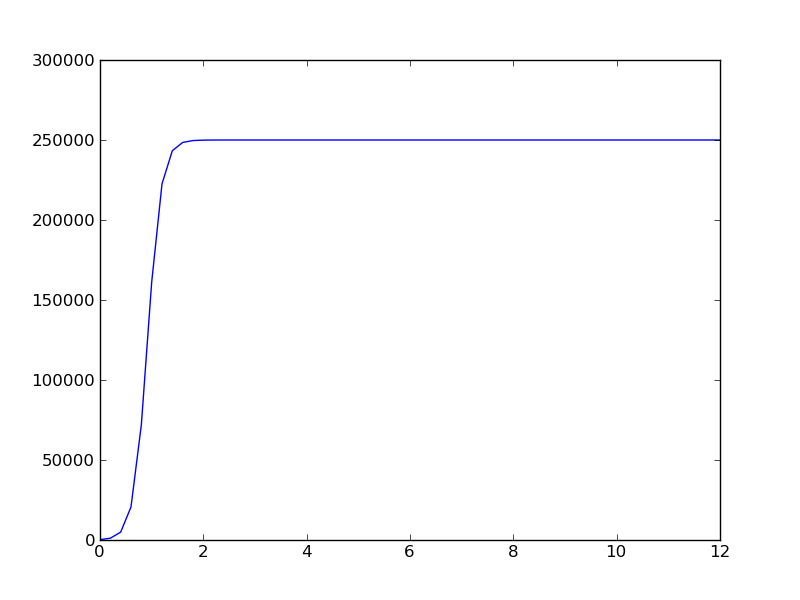
\includegraphics[height=2in, interpolate=true]{data/image}  
\end{center}
\end{frame}


\begin{frame}[fragile]
\frametitle{ODEs - Simple Pendulum}
We shall use the simple ODE of a simple pendulum. 
\begin{equation*}
\ddot{\theta} = -\frac{g}{L}sin(\theta)
\end{equation*}
\begin{itemize}
\item This equation can be written as a system of two first order ODEs
\end{itemize}
\begin{align}
\dot{\theta} &= \omega \\
\dot{\omega} &= -\frac{g}{L}sin(\theta) \\
 \text{At}\ t &= 0 : \nonumber \\
 \theta = \theta_0(10^o)\quad & \&\quad  \omega = 0\ (Initial\ values)\nonumber 
\end{align}
\end{frame}

\begin{frame}[fragile]
\frametitle{ODEs - Simple Pendulum \ldots}
\begin{itemize}
\item Use \typ{odeint} to do the integration
\end{itemize}
\begin{lstlisting}
In []: def pend_int(initial, t):
  ....     theta, omega = initial
  ....     g, L = 9.81, 0.2
  ....     f=[omega, -(g/L)*sin(theta)]
  ....     return f
  ....
\end{lstlisting}
\end{frame}

\begin{frame}[fragile]
\frametitle{ODEs - Simple Pendulum \ldots}
\begin{itemize}
\item \typ{t} is the time variable \\ 
\item \typ{initial} has the initial values
\end{itemize}
\begin{lstlisting}
In []: t = linspace(0, 10, 101)
In []: initial = [10*2*pi/360, 0]
\end{lstlisting} 
\end{frame}

\begin{frame}[fragile]
\frametitle{ODEs - Simple Pendulum \ldots}
%%\begin{small}
\typ{In []: from scipy.integrate import odeint}
%%\end{small}
\begin{lstlisting}
In []: pend_sol = odeint(pend_int, 
                         initial,t)
\end{lstlisting}
\end{frame}

\begin{frame}[fragile]
\frametitle{Result}
\begin{center}
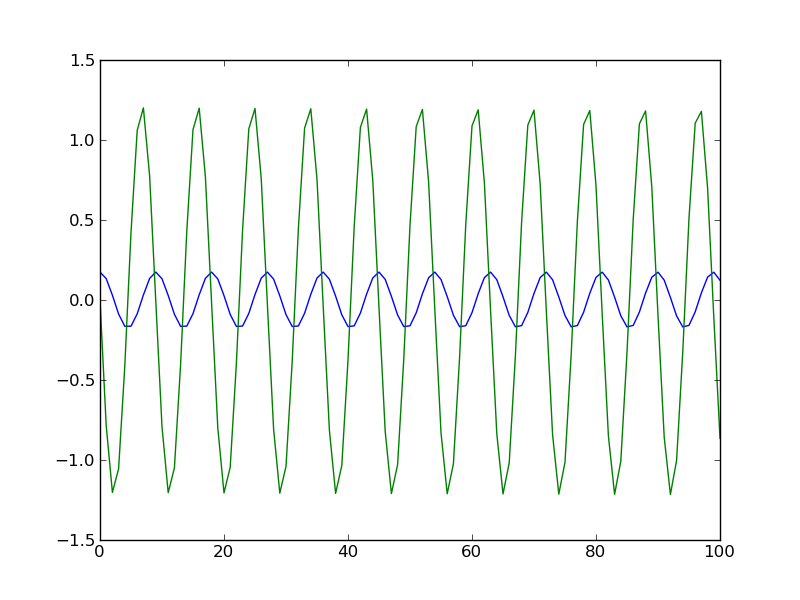
\includegraphics[height=2in, interpolate=true]{data/ode}  
\end{center}
\end{frame}

\begin{frame}
  \frametitle{Things we have learned}
  \begin{itemize}
  \item Solving Linear Equations
  \item Defining Functions
  \item Finding Roots
  \item Solving ODEs
  \end{itemize}
\end{frame}

\end{document}
